\documentclass{beamer}

\usepackage[utf8]{inputenc}
\usepackage[T1]{fontenc}
\usepackage[ngerman]{babel}
\usepackage{graphicx} % Bilder
\usepackage{wrapfig} % Umflussbilder
\usepackage{multicol} % Multiple columns
\usepackage{minted} % Haskell source code
\usepackage{framed} % Frames around source code
\usepackage[framemethod=tikz]{mdframed} % Frames
\usepackage{verbatim} % \begin{comment}...\end{comment}
\usepackage{etoolbox} % manipulate minted
\AtBeginEnvironment{minted}{\fontsize{10}{10}\selectfont}
\AfterEndEnvironment{minted}{}

\mdfdefinestyle{fancy}{
  roundcorner=5pt,
  linewidth=4pt,
  linecolor=red!80,
  backgroundcolor=red!20
}
\newmdenv[style=fancy]{important}

% redifine \em for \emph to use bold instead of italics
\makeatletter
\DeclareRobustCommand{\em}{%
  \@nomath\em \if b\expandafter\@car\f@series\@nil
  \normalfont \else \bfseries \fi}
\makeatother

% Stuff for Beamer
\beamertemplatenavigationsymbolsempty
\usetheme{Warsaw}

\title{Fortgeschrittene Funktionale Programmierung in Haskell}

\begin{document}
  
%----------------------------------------------------------------------------------------  

  \begin{frame}
  \begin{center}
    \huge\textbf{Fortgeschrittene Funktionale Programmierung in Haskell}\\ \bigskip
    \LARGE Universität Bielefeld, Sommersemester 2015\\ \bigskip
    \large Jonas Betzendahl \& Stefan Dresselhaus
    \end{center}
  \end{frame}

%----------------------------------------------------------------------------------------  
\begin{frame}[allowframebreaks]{Outline}
\vfill
Übersicht für Heute:\smallskip

\tableofcontents
\end{frame}

\section{Wiederholung}

%----------------------------------------------------------------------------------------

\begin{frame}

\begin{center}
\Large
\textbf{Wiederholung}
\end{center}

\end{frame}

%----------------------------------------------------------------------------------------

\begin{frame}

\textbf{Leseempfehlung:}

\begin{center}
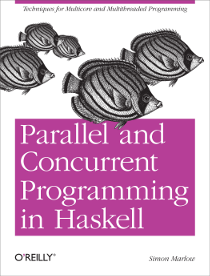
\includegraphics[scale=0.5]{../Woche6/parcur.png} 
\end{center}
\pause

\dots srsly!

\end{frame}

%----------------------------------------------------------------------------------------

\begin{frame}

\begin{center}
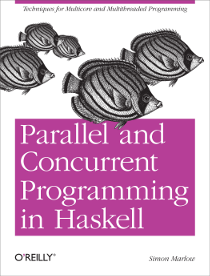
\includegraphics[scale=1]{../Woche6/parcur.png} 
\end{center}

\end{frame}

%----------------------------------------------------------------------------------------

\begin{frame}

\textbf{Überblick:}
\pause

\begin{multicols}{2}
\textbf{Parallelism:}
\begin{itemize}
\item Mehrere Hardwareelemente\pause
\item Antwort schneller kriegen\pause
\item deterministisch (i.d.R.)\pause
\item oft deklarativ\pause
\end{itemize}
\columnbreak
\textbf{Concurrency:}
\begin{itemize}
\item Mehrere Threads\pause
\item Dinge gleichzeitig tun\pause
\item nichtdeterministisch\pause
\item oft impertativ
\end{itemize}
\end{multicols}

\end{frame}

%----------------------------------------------------------------------------------------

%----------------------------------------------------------------------------------------

\section{Threads, MVars, etc.}

\begin{frame}

\begin{center}
\Large
\textbf{Die Basics: Threads, MVars, etc.}
\end{center}

\end{frame}

%----------------------------------------------------------------------------------------

\begin{frame}[fragile]

Wir beginnen mit der Funktion, die einen neuen Thread erstellt:

\mint{haskell}|forkIO :: IO () -> IO ThreadId|
\pause

Threads interagieren notwendigerweise mit der Welt, ergo ist die Berechnung, die wir 
übergeben vom Typ \texttt{IO ()}.\smallskip\smallskip
\pause

Die \texttt{ThreadId} kann später benutzt werden um z.B. den Thread vorzeitig zu töten oder ihm
eine Exception zuzuschmeißen.
\end{frame}

%----------------------------------------------------------------------------------------

\begin{frame}[fragile]

Ein kleines Beispiel:

\begin{minted}{haskell}
import Control.Concurrent
import Control.Monad
import System.IO

main :: IO ()
main = do
  hSetBuffering stdout NoBuffering
  forkIO (replicateM_ 100000 (putChar 'A')) 
  replicateM_ 100000 (putChar 'B')
\end{minted}
\pause
\dots Output?
\pause
\begin{verbatim}
AAAAAAAAABABABABABABABABABABABABABABABABABABABABABABAB
ABABABABABABABABABABABABABABABABABABABABABABABABABABAB
ABABABABABABABABABABABABABABABABABABABABABABABABABABAB
ABABABABABABABABABABABABABABABABABABABABABABABABABABAB
\end{verbatim}
\end{frame}

%----------------------------------------------------------------------------------------

\begin{frame}[fragile]

Aber\dots \pause wie kriegen wir jetzt Ergebnisse aus der Berechnung raus?\\
Der Typ ist nur \texttt{IO ()}, das liefert nichts (interessantes) zurück!\pause\bigskip

Das gleiche Problem hatten wir schon in der \texttt{Par}-Monade. Lösung damals waren
\texttt{IVar}s:\bigskip

\begin{minted}{haskell}
data IVar a  -- instance Eq

new :: Par (IVar a)
put :: NFData a => IVar a -> a -> Par ()
get :: IVar a -> Par a
\end{minted}
\end{frame}

%----------------------------------------------------------------------------------------

\begin{frame}[fragile]

Introducing: \dots \pause \texttt{MVar}s!\bigskip

\begin{minted}{haskell}
data MVar a  -- abstract

newEmptyMVar :: IO (MVar a)
newMVar      :: a -> IO (MVar a)
takeMVar     :: MVar a -> IO a
putMVar      :: MVar a -> a -> IO ()

readMVar     :: MVar a -> IO a
\end{minted}
\pause

Wir brauchen hier keine eigene Monade wie \texttt{Par}. Da Concurrency so oder so
effektvoll ist, reicht \texttt{IO} vollkommen aus.\bigskip

Unterschied zwischen \texttt{IVar}s und \texttt{MVar}s: erstere sind \emph{\textbf{i}}mmutable,
letztere sind \emph{\textbf{m}}utable.

\end{frame}

%----------------------------------------------------------------------------------------

\begin{frame}[fragile]

Ein Beispiel zu \texttt{MVar}s:

\begin{minted}{haskell}
main :: IO ()
main = do
  m <- newEmptyMVar
  forkIO $ do putMVar m 'x'; putMVar m 'y'
  r <- takeMVar m
  print r
  r <- takeMVar m
  print r
\end{minted}
%$
\pause

Wie wir sehen kann die gleiche \texttt{MVar} über Zeit mehrere Zustände annehmen
und erfolgreich zur Kommunikation zwischen Threads benutzt werden. 

\end{frame}

%----------------------------------------------------------------------------------------

\begin{frame}
Generell haben \texttt{MVar}s drei Hauptaufgaben:\pause

\begin{itemize}
\item \textbf{Channel mit nur einem Slot}\\
Eine \texttt{MVar} kann als Nachrichtenkanal zwischen Threads benutzt werden, allerdings maximal eine Nachricht auf einmal halten.\pause

\item \textbf{Behältnis für shared mutable state}\\
In Concurrent Haskell brauchen oft mehrere Threads Zugriff auf einen shared state. Ein beliebtes Designpattern ist, das dieser State als normaler (immutable) Haskell-Datentyp repräsentiert und in einer \texttt{MVar} verpackt wird.\pause

\item \textbf{Baustein für kompliziertere Strukturen}
\end{itemize}
\end{frame}

%----------------------------------------------------------------------------------------

\section{Software Transactional Memory}

\begin{frame}

\begin{center}
\Large
\textbf{Software Transactional Memory (STM)}
\end{center}

\end{frame}

%----------------------------------------------------------------------------------------

\section{Parallelism through concurrency}

\begin{frame}

\begin{center}
\Large
\textbf{Parallelism through Concurrency}
\end{center}

\end{frame}

%----------------------------------------------------------------------------------------

\section{Distributed Programming}

\begin{frame}

\begin{center}
\Large
\textbf{Distributed Programming}
\end{center}

\end{frame}

\end{document}
